%%%%%%%%%%%%%%%%%%%%%%%%%%%%%%%%%%%%%%%%%%%%%%%%%%%%%%%%%%%%%%%%%%%%%%%%%%%%%%%%

\section{Multiple Hypothesis Testing}

When you perform a hypothesis test, it has some probability, $\alpha$, of rejecting the null when, in fact, the null is true. For one test this is manageable. However, when you perform multiple tests, the chance quickly becomes very high that you will reject the null at least once when it's true (a false positive). If you test a lot of hypotheses and don't correct your significance level to account for that, you're likely going to end up with many, many false positives.

\subsection{An Experiment}

Imagine you take random samples of size $40$ in one of two ways, decided by the flip of a [fair] coin. You either (heads) take two groups of $20$ samples each, both from the green distribution (below) or you take one group of $20$ from the green distribution and the other $20$ from the black [dashed] distribution. The difference in means between the two distributions here is 0.5. 

\begin{center}
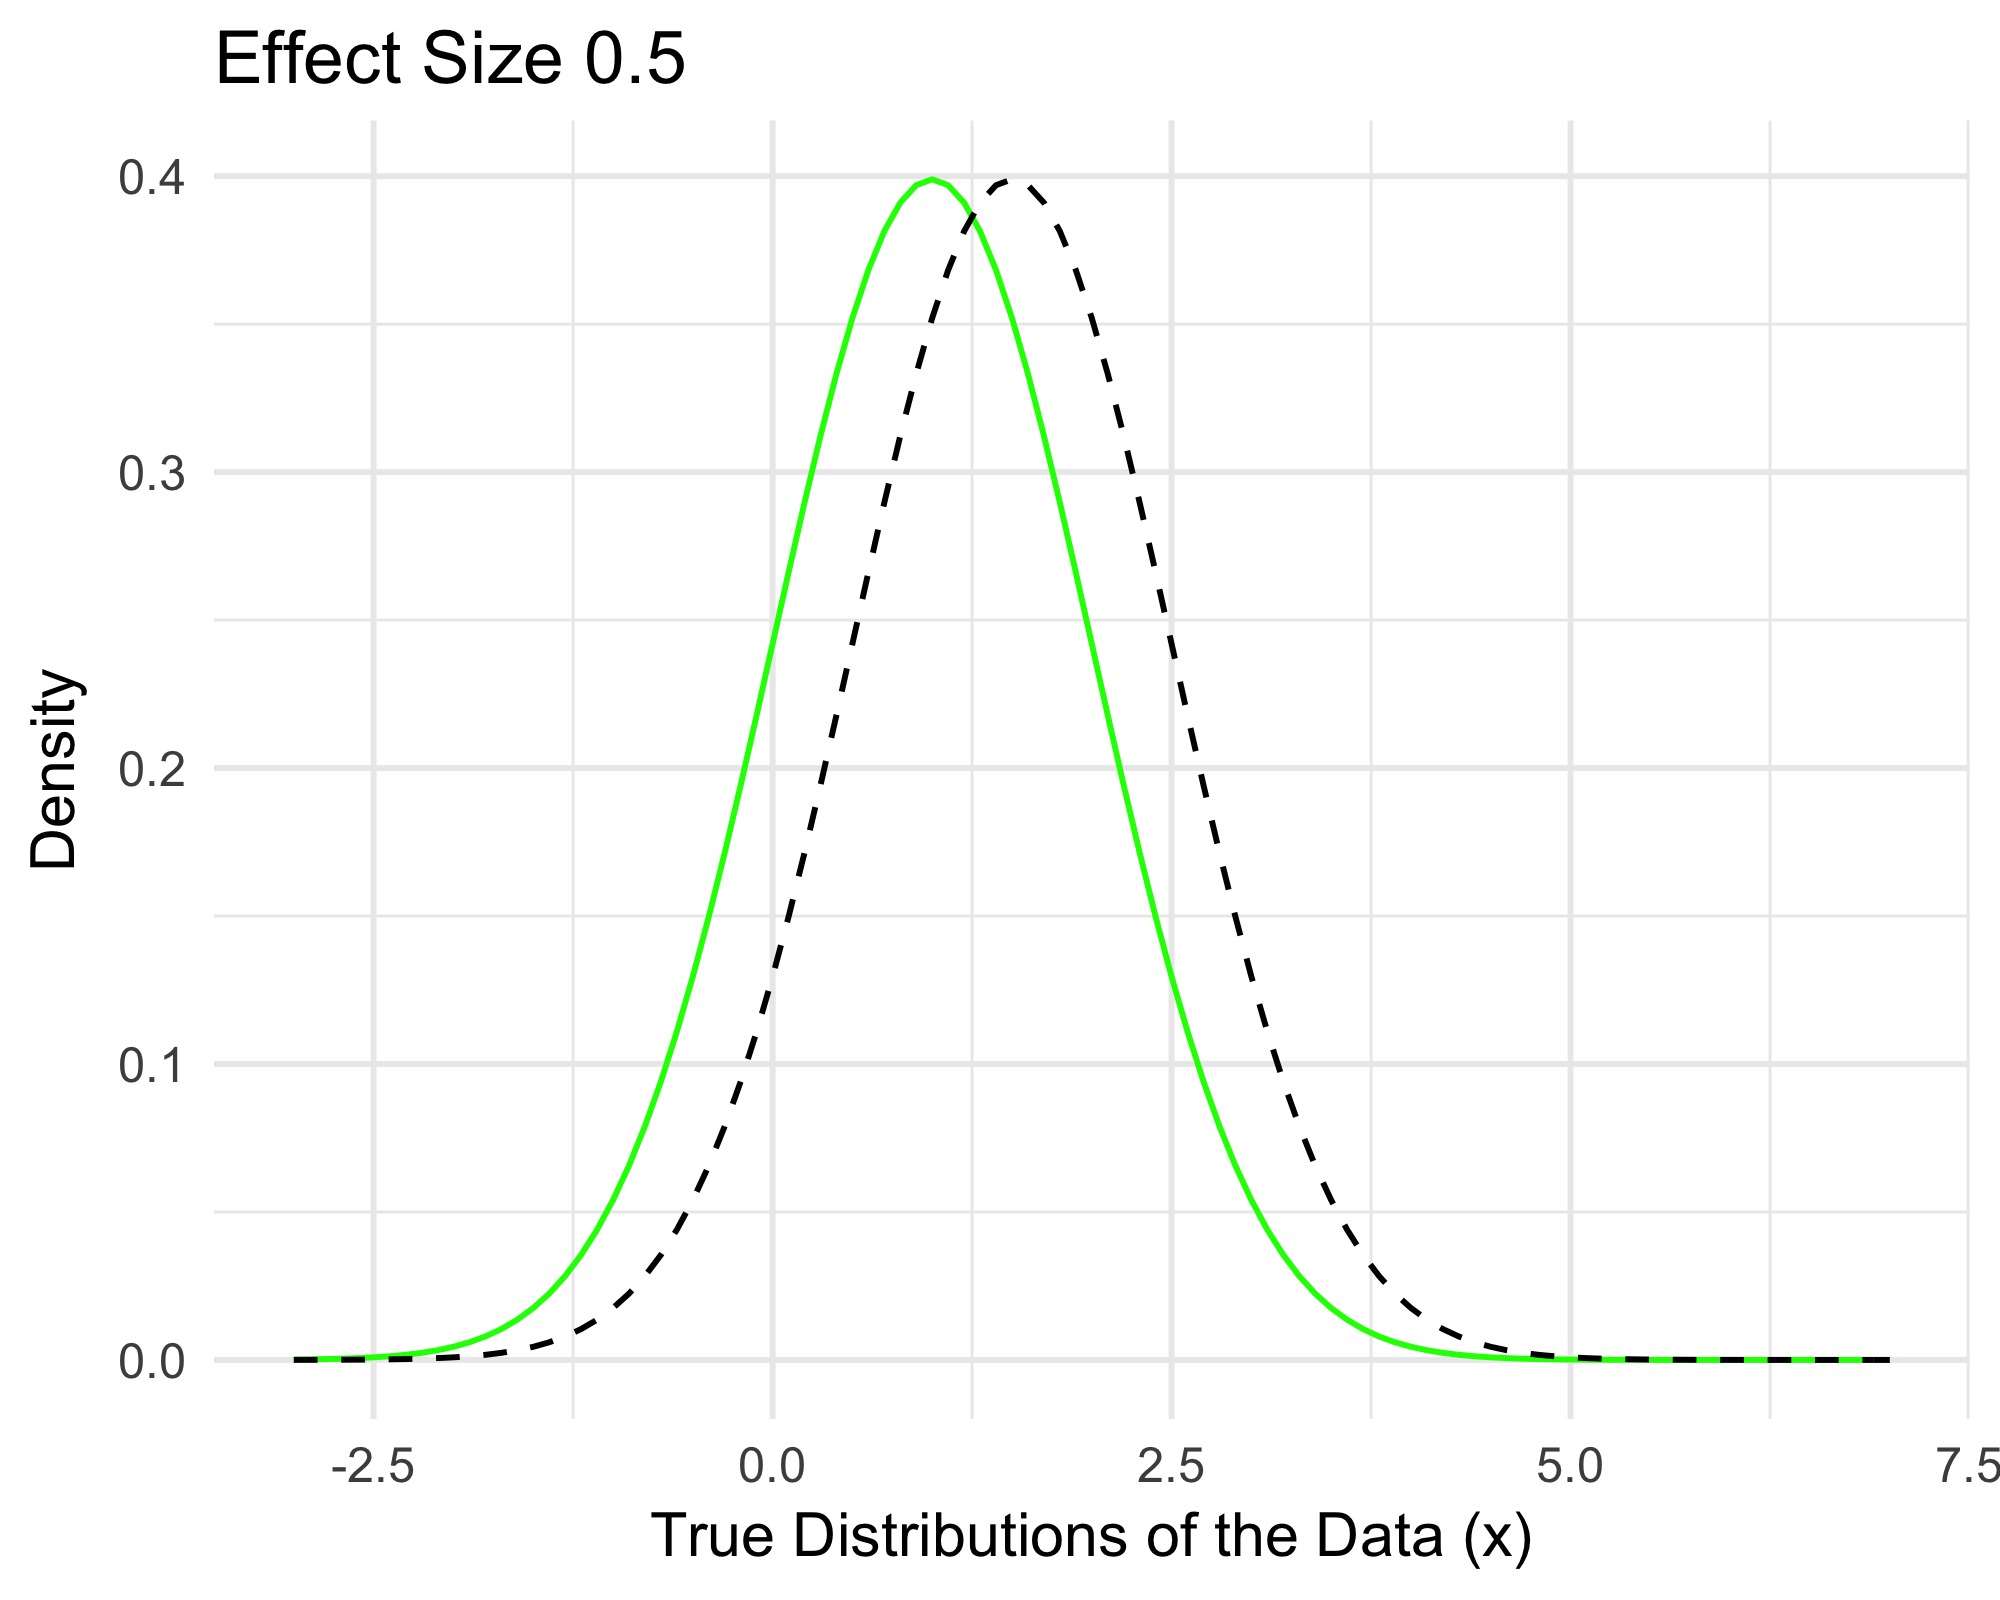
\includegraphics[width=0.6\textwidth]{img/multiple-hypothesis-example-2a.png}
\end{center}

Imagine doing this $10000$ times and, for each run, performing a $T$-test between the two samples. If the $p$-value for that test is below the significance level, $\alpha$, reject the null. Now, measure the fraction of simulations for which the null is rejected and both samples were taken from the same distribution (false positives) and divide that by the total number of simulations where the null was rejected (true positives + false positives). That quotient is the \textbf{False Discovery Rate (FDR)}. Here's how it varies in this experiment with respect to $\alpha$ and effect size: 

\begin{center}
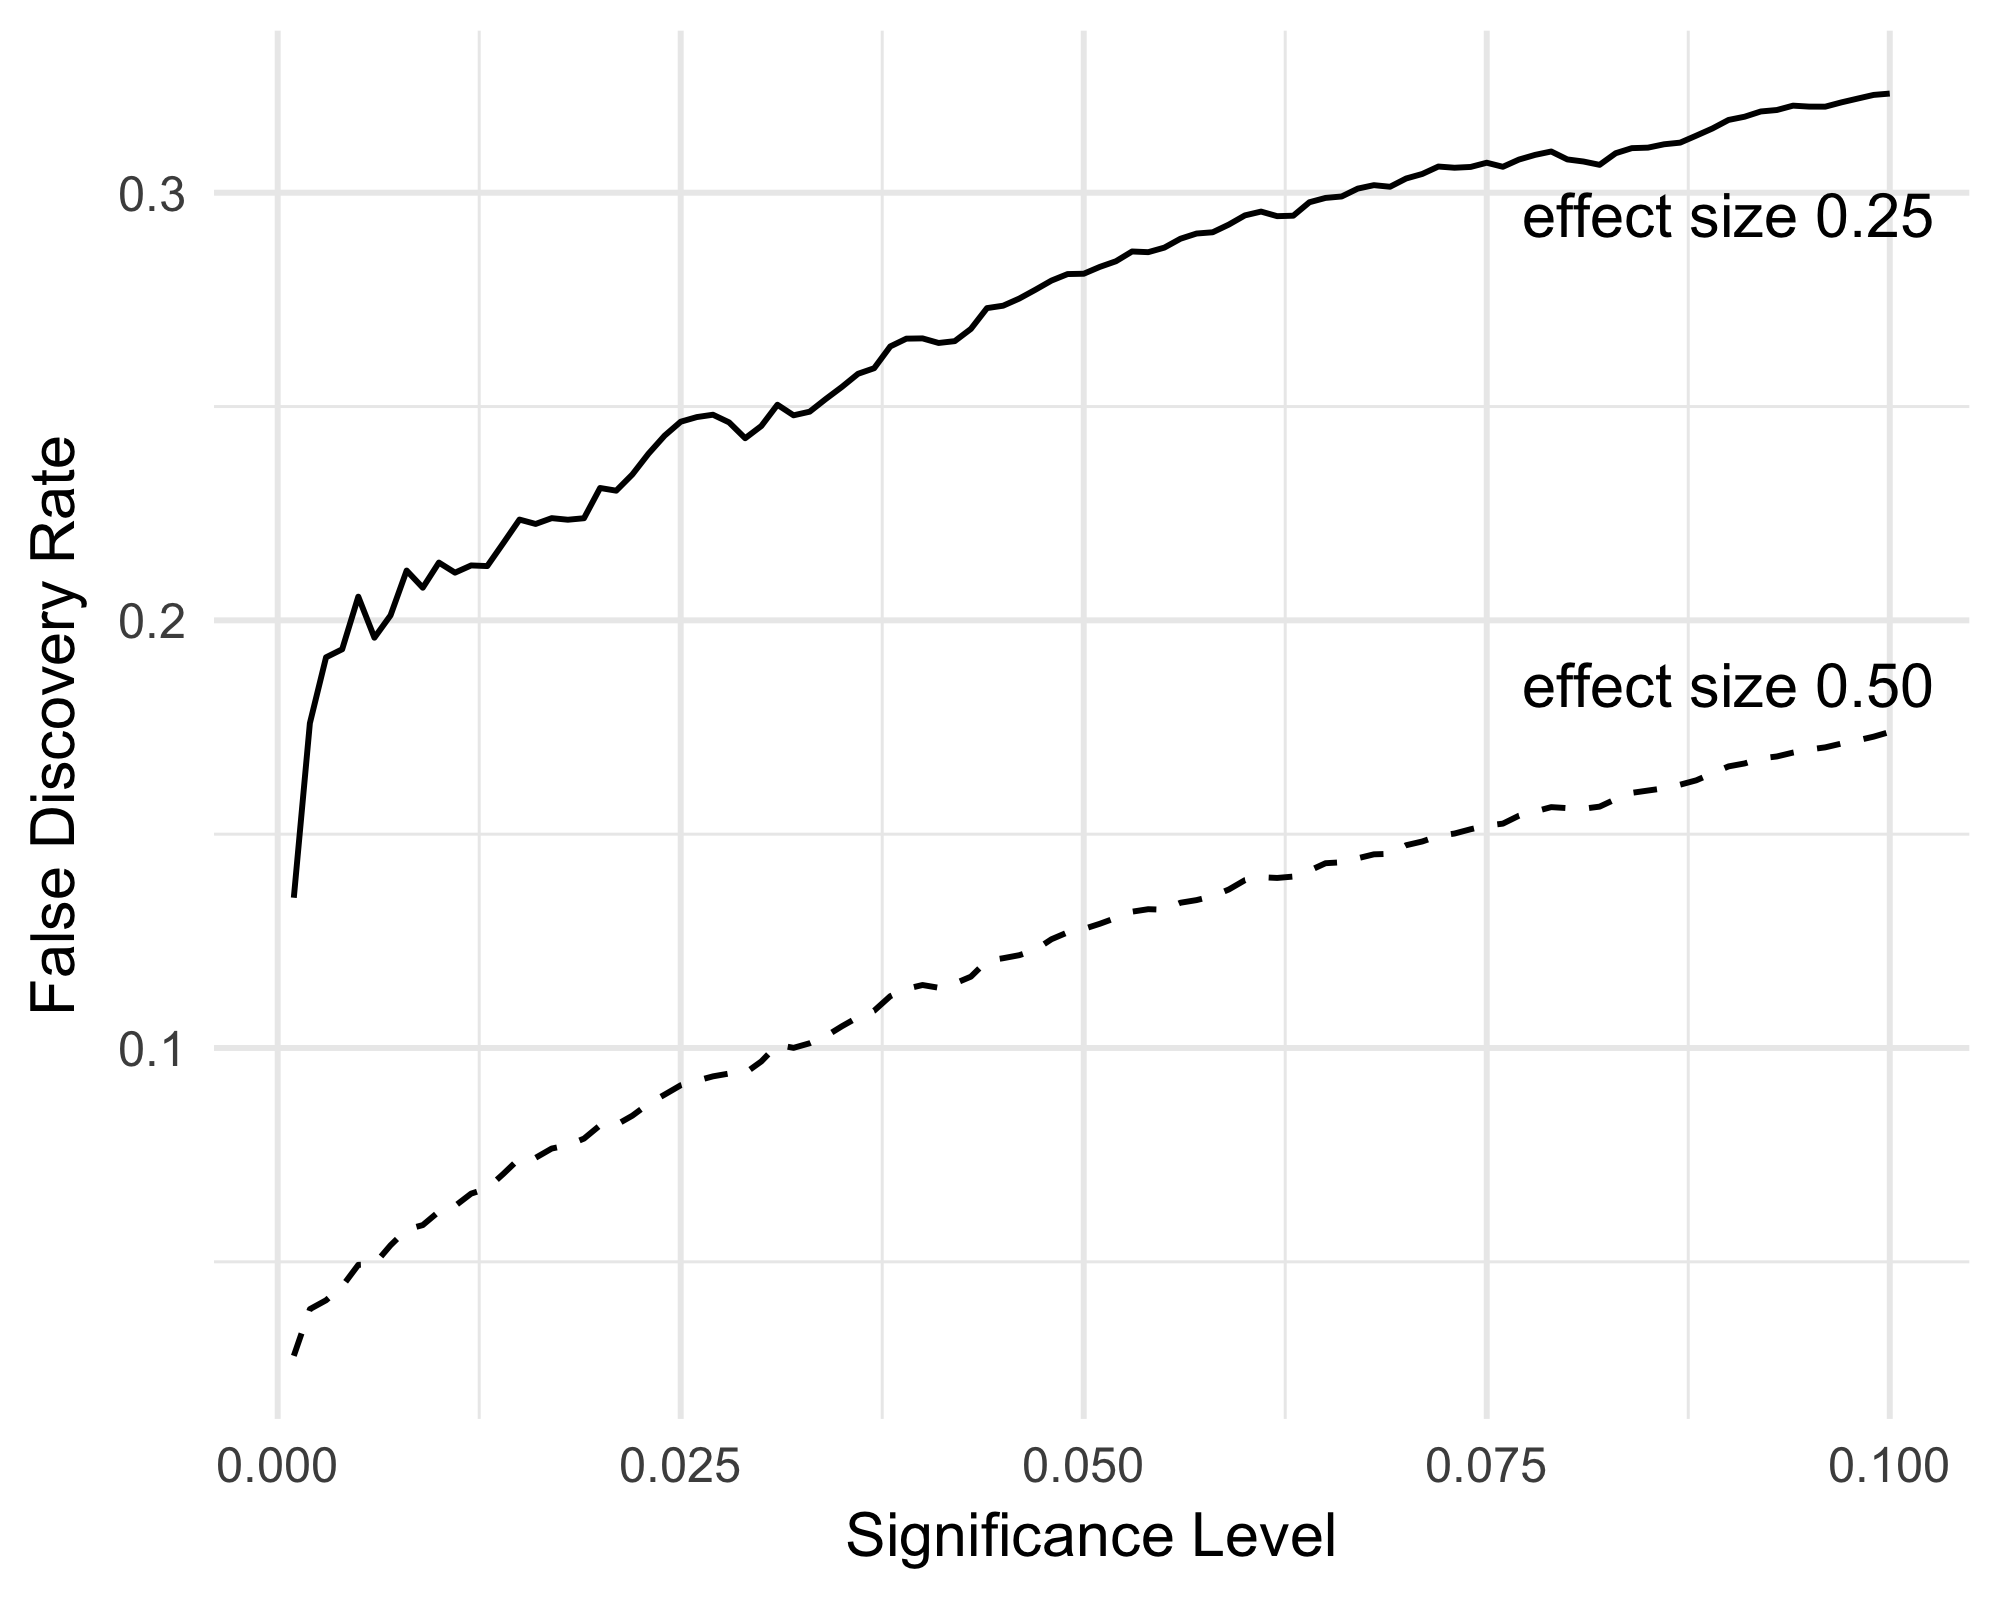
\includegraphics[width=0.6\textwidth]{img/multiple-hypothesis-example-1.png}
\end{center}

\begin{mdframed}
\textbf{Question 2.9:} If the FDR decreases monotonically with decreasing significance level, why not just set $\alpha = 0.0000000001$ or something to minimize FDR?
\vspace{20mm}
\end{mdframed}

There are several algorithms that have been developed and proven to control FDR even though it's impossible to know what the true underlying distribution of effect sizes is. One is called the \textbf{Benjamini-Hochberg} method. Look that up and compare it to the \textbf{Bonferroni correction}, which controls - not the FDR - but the FWER (the probability that at least one significant result is a false positive). 
